\section{weak solutions of elliptic pde}

\begin{example}
	\begin{align}\label{poisson}
	-\laplace u &= f \qquad \text{in } \Omega \\
	u &= 0 \qquad \text{on } \partial \Omega \nonumber
	\end{align}
	
	$\Omega \subset \R^d $ ($d \geq 1$), $\partial \Omega \in C^{0,1}$
\end{example}

If $f \in L^2(\Omega)$, $u \in C^2(\Omega)\cap C(\overline{\Omega})$ is \glqq classical \grqq solution of (\ref{poisson}). Now multiply with $v \in C^\infty_0 (\Omega)$ and integrate by parts.

\begin{align*}
	\int \limits_\Omega fv \diff x &= \int \limits_\Omega \laplace uv \diff x\\
								   &= \int \limits_\Omega \nabla u \cdot \nabla v \diff x - \underbrace{\int \limits_{\partial \Omega} \left( \nabla uv\right)\cdot \vartheta \diff x}_{=0,\ v|_{\partial \Omega} = 0} \\
								   &= \int \limits_\Omega \nabla u \cdot \nabla v \diff x
\end{align*}

Because $C^\infty_0(\Omega)$ is dense in $H^1_0(\Omega)$ this also holds for all $v \in H^1_0(\Omega)$. Now define the Hilbert form
\begin{equation*}
	a(u,v) = \int \limits_\Omega \nabla u \cdot \nabla v \diff x \qquad u,v\in H^1_0(\Omega)
\end{equation*}
and linear functional

\begin{equation*}
	F(v) = \int \limits_\Omega fv \diff x \qquad v \in H^1_0(\Omega).
\end{equation*}

Now we call 
\begin{equation}\label{weak_form}
	a(u,v) = F(v) \qquad \forall v \in  H^1_0(\Omega)
\end{equation}
\textbf{weak formulation} of (\ref{poisson}).\\

We call u
\begin{enumerate}[label=(\alph*)]
\item \textbf{weak solution}, if $u \in  H^1_0(\Omega)$ and $u$ is solution of \eqref{weak_form}
\item \textbf{classical solution} of (\ref{poisson}), if it is also a weak solution of \eqref{weak_form}. 
\end{enumerate}

If $u$ is a weak solution of \eqref{weak_form} and $u \in C^2(\Omega)\cap C(\overline{\Omega})$, u is a classical solution of (\ref{poisson}) Because for $v \in C^\infty_0(\Omega) \subset H^1_0(\Omega)$
\begin{equation*}
	\int \limits_\Omega \left( f + \laplace u \right) v \diff x = \int \limits_\Omega  fv - \nabla u \cdot \nabla v \diff x = 0
\end{equation*}

$\implies \forall v\in L^2(\Omega):$ 
\begin{equation*}
	\int \limits_\Omega \left( f + \laplace u \right) v \diff x = 0.
\end{equation*}

$\implies f + \laplace u = 0$ almost everywhere in $\Omega$.\enter
Because $u \in H^1_0(\Omega)$, there exists $\gamma(u) = 0 = u|_{\partial \Omega}$.

\begin{definition_}
	$V$ is a real Hilbert space, $a: V \times V \to \R$ bilinearform
	\begin{enumerate}[label=(\alph*)]
		\item $a$ is \textbf{continuous} in $V$ if there exists $K > 0$ s.t. $\forall u,v \in V:$ 
		\begin{equation*}
			|a(u,v)| \leq K \|u\|_V \|v\|_V.
		\end{equation*} 
		\item $a$ is \textbf{coercive} (or elliptic) in $V$ if there exists $\lambda > 0$ s.t. $\forall u \in V:$
		\begin{equation*}
			a(u,u)  \geq \lambda \|u\|^2_V
		\end{equation*}
	\end{enumerate}
\end{definition_}

\begin{thrm}
	(Lax-Milgram )\enter
	$V$ real Hilbert space, $a: V \times V \to \R$ is continuous and coercive, $F:V \to \R$. Then there exists a unique solution $u \in V$, s.t.
	\begin{equation*}
		a(u,v) = F(v) \qquad \forall v \in V
	\end{equation*}
	and it holds $\|u\|_V \leq \lambda^{-1}\|F\|_{V'}$.
	%%i think F has to be linear 	
\end{thrm}

\begin{reminder}
	(Representation theorem by Riesz)\enter
	$V$ is a real Hilbertspace with $(\cdot,\cdot)$ scalar product and $F \in \textbf{F} \in V'$. It exists a unique $u \in V$ s.t.
	\begin{equation*}
		(u,v) = F(v) \qquad \forall v\in V
	\end{equation*} 
	and $\|u\|_V = \|F\|_{V'}$.
\end{reminder}

\begin{proof_}
	of Lax-Milgram \enter
	$w \in V$. We have $a(w,\cdot) \in V'$ with Riesz there exists $T(w) \in V$ with 
	\begin{equation}\label{lm_proof}
		(T(w),v) = a(w,v) \qquad \forall v \in V
	\end{equation}
	and 
	\begin{equation*}
		\|T(w)\|_V = \|a(w,\cdot)\|_{V'} \leq K \|w\|_V.
	\end{equation*}
	This shows $T: V \to V$ is continuous and because $a(\cdot,\cdot)$ is bilinear also linear.
\end{proof_}

\par
\underline{\textbf{goal}:}
Show $T^{-1}$ exists and is continuous and linear.\enter

\begin{enumerate}[=label=(\alph*)]
	\item \textbf{existence}:\enter If $g \in V$ is a unique solution of 
	\begin{equation*}
	(g,v) = F(v) \qquad \forall v \in V
	\end{equation*}
	with $\|g\|_V = \|F\|_V$ we obtain with \eqref{lm_proof} 
	\begin{equation*}
	a(T^{-1}(g),v) = (g,v) = F(v) \qquad \forall v \in V
	\end{equation*}
	and therefore $u = T^{-1}(g)$. It also holds that it is unique, as for $u_1, u_2 \in V$ two solutions $u$ have 
	\begin{equation*}
	a(u_1 - u_2,v) = 0 \qquad \forall v \in V
	\end{equation*}
	and thus for $v = u_1 - u_2$
	\begin{equation*}
	\lambda \|u_1 - u_2\|^2_V \leq a(u_1 -u_2, u_1 -u_2) = 0
	\end{equation*}
	and therefore $u_1 = u_2$.
	
	\item  $T^{-1}$\textbf{ injectiv}: \enter
	$a(\cdot, \cdot)$ is coercive $\implies \forall u \in V$
	\begin{equation*}
		\lambda \|u\|^2_V \leq (T(u),u) \leq \|T(u)\|_V\|u\|_V
	\end{equation*}
	and thus 
	\begin{equation}\label{inverse}
		\lambda \|u\|_V \leq \|T(u)\|_V
	\end{equation}
	$\implies T^{-1}$ is injective and $T^{-1}: T(V) \to V$ is continuous with
	\begin{equation*}
		\|T^{-1}(v)\|_V \leq \lambda^{-1}\|v\|_V \qquad \forall v \in T(V). 
	\end{equation*}
	We need to show
	\begin{equation*}
		T(V) = V.
	\end{equation*}
	\item $T(V)$ \textbf{is closed}:\enter
	 $(v_n) \subset T(V)$ with $v_n \to v$ for $n \to \infty$ and $v \in V$. To show $v \in T(V)$. By definition of $v_n$ exists a sequence $(u_n) \subset V$ with $v_n = T(u_n) \to v$. With (\ref{inverse}) $(u_n)$ is a Cauchy sequence in $V$ and $V$ complete follows $u_n \to u \in V$ because $T$ continuous, $T(u_n) \to T(w)$ and thus $T(w)=v$ and $v \in T(V)$\enter
	\item $T(V) = V$:\enter
	 Assume $T(V) \neq V$, as $T(V)$ is a closed linear subspace of $V$, it holds 
	\begin{equation*}
		V = T(V) \oplus T(V)^\perp
	\end{equation*}
	with $T(V)^\perp \neq \emptyset$. If $z \in T(V)^\perp $ with $z \neq 0$
	\begin{equation*}
		(T(v),z) = 0 \qquad \forall v \in V,
	\end{equation*}
	it holds with (\ref{lm_proof}) 
	\begin{equation*}
		0 = (T(z),z) = a(z,z) \geq \alpha \|z\|^2_V
	\end{equation*}
	and thus $z = 0$. This is a contradiction.\\
	Now (\ref{inverse}) implies
	\begin{equation*}
		\|u\|_V = \|T^{-1}(g)\|_V \leq \lambda^{-1}\|g\|_V = \lambda^{-1}\|F\|_{V'}.
	\end{equation*}
\end{enumerate}

\textbf{\underline{consider}}
\begin{itemize}
	\item Dirichlet boundary conditions(short BC)\enter
	\item Neumann BC\enter
	\item Robin BC
\end{itemize}


\begin{enumerate}[=(\alph*)]
	\item \textbf{Dirichlet BC}:\enter
	look for weak solutions of 
	\begin{align*}
		Lu &= f \qquad \text{in } \Omega\\
		 u &= g \qquad \text{on } \partial \Omega
	\end{align*}
	with 
	\begin{equation*}
		Lu = - \displaystyle \sum^d_{i,j} \frac{\partial}{\partial x_i} \left(  a_{ij}(x) \frac{\partial u}{\partial x_j} \right) + c(x)u.
	\end{equation*}
	\begin{example}
		\begin{align*}
			d &= 1,&   a_{11}(x)&=1,              & c(x)&=0 \\
			  &    &            &				  &     &  \\
			d &= 2,&   a_{11}(x)&= a_{22}(x) = 1, & c(x)&=0 \\ 
			  &    &   a_{12}(x)&= a_{21}(x) = 0  &     &   \\
		  	  &    &         Lu &= -\laplace      &     &   \\
		\end{align*}
	\end{example}
	\begin{definition_}
		$L$ is \textbf{elliptic} in $\Omega$ if $\lambda > 0$ exists, s.t. $\forall \xi \in \R^d$ and  $x \in \Omega$
		\begin{equation*}
			\displaystyle \sum^d_{i,j} a_{ij}(x)\xi_i\xi_j \geq \lambda |\xi|^2
		\end{equation*}
	\end{definition_}
	weak form 
	\begin{align*}
		a(u,v) &= \displaystyle \sum_{i,j} \int \limits_\Omega a_{ij}(x)\frac{\partial u}{\partial x_i} \frac{\partial v}{\partial x_j} \diff x + \int \limits_\Omega cuv \diff x \\
		F(v)&= \int \limits_\Omega fv \diff x
	\end{align*}
	Look for $u$ with $u = g \in H^1_0(\Omega)$ and transform equation to homogenous BC. $w = u - g \in H^1_0(\Omega)$ is solution of 
	\begin{align*}
		Lw &= f -Lg \qquad \text{in } \Omega\\
		 w &= 0 \qquad \qquad \ \,\text{on } \partial\Omega.
	\end{align*}
	Define right hand side
	\begin{equation*}
		G(v) = F(v) - \displaystyle \sum^d_{i,j} \int \limits_\Omega a_{ij} \frac{\partial g}{\partial x_j}\frac{\partial v}{\partial x_i} \diff x - \int \limits_\Omega cgv \diff x \quad \forall v\in H^1_0(\Omega).
	\end{equation*}
	Weak formulation: find $w\in H^1_0(\Omega)$ 
	\begin{equation*}
		a(w,v) = G(v) \qquad \forall v \in H^1_0(\Omega)
	\end{equation*}
	$\implies u = w +g$ is weak solution of original problem.
	\begin{comment_}
		$u = g $ on $\partial \Omega$ means $\gamma(u-g) = 0$
	\end{comment_}

	\begin{thrm}
		If $\Omega \subset \R^d\ (d\geq1)$ bounded, $a_{ij},c \in L^\infty(\Omega), c\geq 0, f\in L^2(\Omega), g\in H^(\Omega),\ L$ is elliptic, then there exists a unique solution $u \in H^1(\Omega)$ of $Lu=f$ with  $u-g \in H^1_0(\Omega)$ and 
		\begin{equation*}
			\|u\|_{H^1} \leq C\left( \|f\|_{L^2} \|g\|_{H^1} \right)
		\end{equation*}  
		with $C = C(\lambda, \Omega,a_{ij},c)>0$.
	\end{thrm}

	\begin{proof_}
		Use Lax-Milgram with $V = H^1_0$
		\begin{itemize}
			\item a is continuous:\enter
			Cauchy-Schwartz inequality
			\begin{align*}
				|a(u,v)| &\leq \displaystyle \sum^d_{i,j=1} \int \limits_\Omega |a_{ij}| |\frac{\partial u}{\partial x_i}| |\frac{\partial v}{\partial x_j}| \diff x + \int \limits_\Omega |c||u||v| \diff x \\
				& \leq \underset{i,j = 1,\dots,d}{\max} \Big\{ \|a_{ij}\|_{L^\infty}, \|c\|_{L^\infty} \Big\}\left( \displaystyle \sum^d_{i,j=1} \|\frac{\partial u}{\partial x_j}\| \|\frac{\partial v}{\partial x_i}\| + \|u\|\|v\| \right)\\
				&= K \Big ( \|\nabla u\|_{L^2}\|\nabla v\|_{L^2} + \|u\|_{L^2}\|v\|_{L^2} \Big )\\
				&\leq K \|u\|_{H^1}\|v\|_{H^1}
			\end{align*}
			\item a is coercive: \enter
			$ u \in H^1_0(\Omega), L$ elliptic, $c \geq 0$
			\begin{align*}
				a(u,u) &\geq \lambda \displaystyle\sum^d_{i=1} \int \limits_\Omega |\frac{\partial u}{\partial x_i}|^2 \diff x\\
					   &= \lambda\|\nabla u\|_{L^2}\\
					   &\geq \lambda_0 \|u\|^2_{H^1}
			\end{align*}
			with $\lambda_0 = \frac{\lambda}{C^2_p +1}$ and with poincaré-inequality follows
			\begin{equation*}
				\|u\|^2_{H^1} = \|u\|^2_{L^2} + \|\nabla u\|^2_{L^2} \leq \left( 1 + C^2_p \right)\|\nabla u\|^2_{L^2}.
			\end{equation*}
			\item $G \in V' = H^{-1}(\Omega)$:\enter
			Cauchy-Schwartz inequality
			\begin{align*}
				|G(v)| & \leq \|f\|_{L^2}\|v\|_{L^2} + \underset{i,j=1, \dots, d}{\max} \|a_{ij}\|_{L^\infty} \|\nabla v\|_{L^2} \|\nabla g\|_{L^2} + \|c\|_{L^\infty}\|g\|_{L^2}\|v\|_{L^2}\\
					   & \leq \big (  \|f\|_{L^1} + C_i\|g\|_{H^1} \big ) \|v\|_{H^1}\\ 
			\end{align*}
			with $C_i =  \underset{i,j=1, \dots, d}{\max} \|a_{ij}\|_{L^\infty} + \|c\|_{L^\infty}$
			\begin{equation*}
				\implies  \|G\|_{H^{-1}} \leq \|f\|_{L^2} +  C_i\|g\|_{H^1}
			\end{equation*}
			and because $G \in H^{-1}(\Omega)$ we also have
			\begin{equation*}
				<G,v>_{H^{-1}} = <f-Lg,v>_{H^{-1}} \qquad \forall v \in H^1_0(\Omega).
			\end{equation*}
			Lax-Milgram gives, there exists a unique solution $w \in V$ with $a(w,v) = G(v)\ \forall v \in V$ and for $u = w+g$ we have
			\begin{align*}
				\|u\|_{H^1} & \leq \|w\|_{H^1} + \|g\|_{H^1}\\
							& \leq \lambda^{-1}_0 \left( C^2_p +1 \right)\big (  \|f\|_{L^2} +  C_i\|g\|_{H^1} \big ) + \|g\|_{H^1}\\
							& \leq C \big ( \|f\|_{L^2} + \|g\|_{H^1} \big ) 
			\end{align*}
			with $C = 1+ \lambda^{-1}(C^2_p+1)(C_i +1)$.
		\end{itemize}
	\end{proof_}
	\item \textbf{Neumann BC}:\enter
	consider special case  
	\begin{align*}
		- \laplace u + c(x)u &= f \qquad \text{in }\Omega\\
		\nabla u \cdot \vartheta &=g \qquad \text{on } \partial\Omega
	\end{align*}
	with $c \in L^\infty(\Omega), c\geq 0, f\in L^2(\Omega), g \in H^1(\Omega)$.
	If $u \in C^2(\Omega)\cap C(\overline{\Omega})$ is a classical solution and $c \in C^\infty(\Omega)$.
	\begin{align*}
		\int \limits_\Omega fv \diff x &= \int \limits_\Omega \nabla u \cdot  \nabla v + cuv \diff x - \int \limits_{\partial\Omega} (\nabla u \cdot \vartheta)v \diff s\\
		&= \int \limits_\Omega \nabla u \cdot  \nabla v + cuv \diff x - \int \limits_{\partial\Omega} gv \diff s.
	\end{align*}
	Define 
	\begin{align*}
		a(u,v) &= \int \limits_\Omega \nabla u \cdot  \nabla v + cuv \diff x \qquad \forall u,v\in H^1(\Omega)\\
		F(v) &= \int \limits_\Omega fv \diff x + \int \limits_{\partial\Omega} gv \diff s \qquad \forall v \in H^1(\Omega).
	\end{align*}
	Weak formulation: Find $u \in H^1(\Omega)$, s.t.
	\begin{equation*}
		a(u,v) = F(v) \qquad \forall v \in H^1(\Omega).
	\end{equation*}
	\begin{comment_}
		If $c \equiv 0, -\laplace u=f$ in $\Omega$, $\nabla u\cdot\vartheta = g$ on $\partial \Omega$.
		\begin{align*}
			\int \limits_\Omega f \diff x &= \int \limits_\Omega \text{div}(\nabla u) \diff x\\
			&= -\int \limits_{\partial \Omega} \nabla u \cdot  \vartheta \diff s\\
			&= -\int \limits_{\partial \Omega} g \diff s.
		\end{align*}
		The problem is only solvable if $F(1)=0$. If $u$ is a solution, also $u +$ constant is a solution.\enter
		Lax-Milgram with space $V = H^1(\Omega)$ does not work as $a(u,u)=0$ for constant functions $u \implies a$ is not coercive.\enter
		Use $V = \{ u \in H^1(\Omega), \int \limits_\Omega u \diff x =0 \}$ guarantees uniqueness and excludes constant functions. For $c \neq 0$ it holds 
		\begin{equation*}
			a(u,u) \geq \min\left( \underset{\Omega}{\inf}\ c \right)\|u\|^2_{H^1} 
		\end{equation*}
		and thus coercive.
	\end{comment_}
	\begin{thrm}\enter
		\begin{enumerate}[label=(\Roman*)]
			\item If $\underset{\Omega}{\inf}\ c > 0$, there exists a unique solution $u \in H^1(\Omega)$.
			\item If $c \equiv 0$ and $F(1)=0$ there exists a unique solution $u \in \{ u \in H^1(\Omega): \int \limits_\Omega u \diff x =0 \}$.
		\end{enumerate}
		In both cases there exists $C > 0$ s.t. 
		\begin{equation*}
			\|u\|_{H^1} \leq C \big ( \|f\|_{L^2} + \|g\|_{H^1} \big )	
		\end{equation*}
	\end{thrm}
	\begin{proof_}\enter
		\begin{itemize}
			\item Part (I): \enter
				$a$ is continuous in $V = H^1(\Omega)$: see Dirichlet BC.\enter
				$a$ is coercive:
				\begin{equation*}
					a(u,u) \geq \lambda \|u\|^2_{L^2}
				\end{equation*}
				with $\lambda = \min(1, \underset{\Omega}{\inf}\ c )$.\enter
				$F$ is linear functional
				\begin{align*}
					|F(v)| & \leq \|f\|_{L^2} \|v\|_{L^2} + \|\gamma(g)\|_{L^2(\partial \Omega) } \|\gamma(v)\|_{L^2(\partial \Omega) }\\
					& \overset{*}{\leq} \|f\|_{L^2} \|v\|_{L^2} +C_\gamma \|g\|_{H^1(\Omega)}\|v\|_{H^1(\Omega)}\\
					& \leq \left( \|f\|_{L^2} + +C_\gamma \|g\|_{H^1(\Omega)} \right)\|v\|_{H^1(\Omega)}
				\end{align*}
				$(*)$ holds because of the continuity of the boundary operator. Thus $F \in V'$.\enter
				Lax-Milgram gives existance and uniqueness and also 
				\begin{equation*}
					 \|u\|_{H^1} \leq \lambda^{-1} \|F\|_{V'} \leq \lambda^{-1} \max(1, \C_\gamma)\big (  \|f\|_{L^2} + \|g\|_{H^1} \big )
				\end{equation*}
			\item Part (II): \enter
				we need to prove that $ V = \{ u \in H^1(\Omega): \int \limits_\Omega u \diff x =0 \}$ is Hilbert space and $\|u\|_V = \|\nabla u \|_{L^2}$.\enter
				$a$ is coercive:
				\begin{equation*}
					a(u,u) \geq \|\nabla u\|^2_{L^2} = \|u\|^2_V
				\end{equation*}
				with $\lambda = 1$.\enter
				$a$ is continuous:
				\begin{align*}
					|a(u,v)| &\leq \|\nabla u\|_{L^2}\|\nabla v\|_{L^2} + \|c\|_{L^\infty} \| u\|_{L^2} \|v\|_{L^2}\\
					& \leq \| u\|_{V}\| v\|_{V} + \|c\|_{L^\infty} \| u\|_{H^1} \|v\|_{H^1}\\
					& \leq \| u\|_{V}\| v\|_{V} + C^2_V\|c\|_{L^\infty} \| u\|_{V} \|v\|_{V}\\
					&= \left( 1 + C^2_V \|c\|_{V^\infty} \right) \|u\|_V \|v\|_V.
				\end{align*}
				$F$ is a linear functional: see case above\enter
				Lax-Milgram: existence and uniqueness and continuous dependency on data.
		\end{itemize}
	\end{proof_}
	\item \textbf{Neumann BC}:
	\begin{align*}
				   	  -\laplace u &= f \qquad \text{in }\Omega\\
			 				    u &= 0 \qquad \text{on }\Gamma_D\\
		 \nabla u \cdot \vartheta &= 0 \qquad \text{on }\Gamma_N
	\end{align*}
	with $\partial \Omega = \Gamma_D \cup \Gamma_N$, $ \Gamma_D \cap \Gamma_N = \emptyset$ and meas$(\Gamma_D) >0$.\enter If  meas$(\Gamma_N)>0$ the space $H^1_0(\Omega)$ does not work. $H^1_0(\Omega \cup \Gamma_N)$ = completness of $C^\infty_0(\Omega \cup \Gamma_N)$ in $\|\cdot\|_{H^1}$ with 
	\begin{equation*}
		C^\infty_0(\Omega \cup \Gamma_N) = \{ u \in C^\infty(\overline{\Omega}), \text{supp }u \subset \Omega \cup \Gamma_N  \}.
	\end{equation*}
	Define $\gamma_D: H^1(\Omega) \to L^2(\Gamma_D)$ with $\gamma_D(u) = u|_{\Gamma_D}$ and now use it to represent 
	\begin{equation*}
		H^1_0(\Omega \cup \Gamma_N) = \{ u \in H^1(\Omega): \gamma(u) = 0 \}.
	\end{equation*}
	If $u \in C^2(\Omega) \cap C^1(\overline{\Omega})$ is classical solution and $v \in C^\infty_0(\Omega \cup \Gamma_N)$ then
	\begin{align*}
		\int \limits_\Omega fv \diff x &= \int \limits_\Omega \nabla u \cdot  \nabla v + cuv \diff x - \int \limits_{\partial\Omega} (\nabla u \cdot \vartheta)v \diff s\\
		 &= \int \limits_\Omega \nabla u \cdot  \nabla v + cuv \diff x -   \underbrace{\int \limits_{\Gamma_N} (\nabla u \cdot \vartheta)v \diff s}_{=0,\ \nabla u \cdot \vartheta =0 } - \underbrace{\int \limits_{\Gamma_D} (\nabla u \cdot \vartheta)v \diff s}_{=0,\ v=0 \text{ on } \Gamma_D} \\
	\end{align*}
	\begin{thrm}
		$f \in L^2$, there exists a unique solution $u\in V$ and $\|u\|_{H^1} \leq C\|f\|_{L^2}$ with $C>0$ and
		\begin{equation*}
			V = H^1_0(\Omega \cup \Gamma_N).
		\end{equation*}
	\end{thrm}
	\begin{proof_}
		Use Lax-Milgram.
	\end{proof_}
\end{enumerate}

\subsection{Ritz-Galerkin-Method}
Let $V$ be a real vector space, $a:V\times V \to \R $ continuous bilinearform and $F \in V'$. How to solve
\begin{equation*}
	a(u,v) = F(v) \quad \forall v \in V \text{ with }u \in V
\end{equation*}
approximatly?\\
\underline{Idea:} consider finite dimensional space $V_h \subset V$ ($h > 0$, related to grid spacing)\\
\underline{Ritz-Galerkin approximation}
\begin{equation*}
	a(u_h,v) = F(v) \quad \forall v \in V_h \text{ with }u \in V_h
\end{equation*}
Now consider $\{ \varphi_1,\dots,\varphi_N\}$ basis of $V_h$ and now
\begin{equation*}
	a(u_h,\varphi_i) = F(\varphi_i) \quad \forall i = 1, \dots,N.
\end{equation*}
In addition 
\begin{equation*}
	u_h = \displaystyle \sum^N_{j=1} u_j\varphi_j
\end{equation*}
implies
\begin{equation*}
	\displaystyle \sum^N_{j=1} u_ja(\varphi_j, \varphi_i) = F(\varphi_i) \quad \forall i = 1, \dots,N.
\end{equation*}
We have $N$ unknowns $u_1,\dots,u_N$ and with the notation
\begin{align*}
	A &= (A_{ij}) = (a(\varphi_j, \varphi_i))\\
	b &= (F(\varphi_i))\\
	u &=(u_i)
\end{align*}
we obtain
\begin{equation*}
	Au =b.
\end{equation*}
$A$ is called \glqq stiffness matrix\grqq\ and $b$ is called \glqq load vector\grqq.
If $a(\cdot,\cdot)$ is coercive in $V$, then it is also coercive in $V_h \implies$ linear system has a unique solution. 
\begin{align*}
	\forall \xi \in \R^N, z &:= \displaystyle \sum^N_{i=1} \xi\varphi_i\\
	\xi^TA\xi &= \displaystyle \sum^N_{i,j=1}a(\varphi_j,\varphi_i)\xi_j\xi_i\\
	&=a(z,z)\\
	& \geq \lambda \|z\|^2_V.
\end{align*}
\begin{equation*}
	A\xi = 0 \implies z=0 \implies \xi = 0.
\end{equation*}
A is injectiv, invertable $\implies$ unique solution.
\begin{lemma_}
	(Lemma of Cea)\\
	$V$ Hilbert space,$a(\cdot,\cdot)$ continuous, coerciv, bilinearform on $V$, $F \in V'$,$V_h \subset V$.\\
	$u\in V$ is solution of $a(u,v) = F(v) \forall v\in V$\\
	$u_h\in V_h$ is solution of $a(u_h,v) = F(v) \forall v\in V_h$\\
	\begin{equation*}
		\implies \|u-u_h\|_V \leq \frac{K}{\alpha}\underset{v \in V_h}{\inf}\|u-v\|_V
	\end{equation*} 
	with $K,\lambda$ constants from continuity and coercivity inequalities.
\end{lemma_}
\begin{proof_}
	Subtract $a(u,v) = F(v)$ and $a(u_h,v) = F(v)$ with $v \in V_h$.
	\begin{equation*}
		\implies a(u-u_h,v)=0\quad \forall v\in V_h
	\end{equation*}
	use $v-u_h \in V_h$ and we obtain
	\begin{equation}\label{cea}
		a(u-u_h,v-u_h)=0\quad \forall v\in V_h.
	\end{equation}
	Now
	\begin{align*}
		\lambda \|u-u_h\|^2_V &\leq a(u-u_h,u-u_h)\\
		&= a(u-u_h,u-v) + \underbrace{a(u-u_h,v-u_h)}_{\overset{\ref{cea}}{=}0}\\
		&= a(u-u_h,u-v)\\
		&\leq K\|u-u_h\|_V\|u-v\|_V.
	\end{align*}
	\begin{equation*}
		\implies \|u-u_h\|_V \leq \frac{K}{\alpha}\|u-v\|_V \quad \forall v\in V_h.
	\end{equation*}
\end{proof_}
If $a$ is symmetric, $a(u,v) = a(v,u) \forall u,v \in V$, $a$ is a scalar product on $V$ (and $V_h$).\\
geometric approximation of Cea-lemma: $u-u_h$ is orthogonal to $V_h,u_h$ is the element in $V_h$ \glqq closest\grqq to u. To get $u_h \to u$ for $h \to 0$ we need $V_h \to V$ if $h\to 0$. If 
\begin{align*}
	\underset{h\to 0}{\text{lim}} \text{ dist}(u,V_h) &= 0 \quad \forall u \in V\\
	\implies \underset{h\to 0}{\text{lim}}\|u-u_h\|_V &=0.
\end{align*}
If $a(\cdot,\cdot)$ is symmetric, we can write the problem as a minimization problem.
\begin{lemma_}
	Same conditions as for Cea-lemma and $a$ symmetric. The following statements are equivalent:
	\begin{enumerate}[label=(\alph*)]
		\item \label{variation_1} $a(u,v)= F(v) \quad \forall v\in V$ 
		\item \label{variation_2} $E(u) = \underset{v \in V}{\min}E(v) $ with $E(v) = a(v,v) -2F(v)$.
	\end{enumerate}
\end{lemma_}

\begin{proof_}
	$v \in V$, define $e:\R \to \R$:
	\begin{equation*}
		e(t) = E(u+tv) \overset{taylor}{=} E(u) + 2t\big ( a(u,v) - F(v)\big ) +t^2 a(v,v)  .
	\end{equation*}
	\begin{itemize}
		\item  \ref{variation_2} $\implies$  \ref{variation_1}:\\
			$u$ is solution of \ref{variation_2}, $e$ has minimum at $t=0$
			\begin{equation*}
				e'(0)=0 \implies a(u,v)=F(v)
			\end{equation*} 
		\item \ref{variation_1} $\implies$  \ref{variation_2}:\\
			$u$ is solution of \ref{variation_1} implies
			\begin{equation*}
				E(u) \leq \underbrace{E(u) + a(v,v)}_{= e(1)} = E(u,v).
			\end{equation*}
			with $v = v-u \implies E(u) \leq E(v)$
	\end{itemize}
\end{proof_}

Allows to interprete the discrete problem 
\begin{equation*}
	a(u_h,v) = F(v)
\end{equation*}
as finding a minimum of $E$ not in V but in \glqq smaller\grqq space $V_h$. $E$ can be seen as energy and $a(u_h,v) = F(v)$ as the Euler-Lagrange-equation of this energy. 
\begin{equation*}
	Au=b \quad \text{or} \quad \min E(u_h)
\end{equation*}
\par
What is needed to solve the weak form or Ritz-Galerkin-approximation?
\begin{itemize}
	\item compute coefficients $A_{ij} = a(\varphi_j,\varphi_i)$
	\item solve the linear system
\end{itemize}

\underline{goal}: have computation of $A_{ij}$ as simple as possible. $A$ should ontain many zeros, $A$ should be a sparse matrix.

\section{Finite-Flements}
consists of 3 characteristics:
\begin{itemize}
	\item $\overline{\Omega}= \underset{\tau \in \T_h}{\bigcupdot} \tau$\quad  with $\tau$ triangles, rectangles in $\R^2$ or tetraheder in $\R^3$
	\begin{figure}[h!]
	\center

	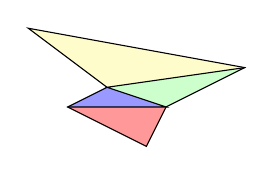
\begin{tikzpicture}[scale=1]
	
	
	% fill triangles
	\fill[red!40!white]   (0,0) -- ++(1,-0.5) -- ++(0.25,0.5) --cycle;
	\fill[blue!40!white]  (0,0) -- ++(1.25,0) --++(-0.75,0.25) --cycle;
	\fill[green!20!white]   (1.25,0) --++(-0.75,0.25) --++(1.75,0.25) --cycle;
	\fill[yellow!20!white]   (0.5,0.25) --++(1.75,0.25) --  ++(-2.75,0.5) --cycle;
	
	% outline
	\draw (0,0) -- ++(1,-0.5) -- ++(0.25,0.5)-- ++(1,0.5) -- ++(-2.75,0.5)-- ++(1,-0.75)--cycle;
	
	% this is unrobust
	\draw (0,0) -- ++(1.25,0) --++(-0.75,0.25) --++(1.75,0.25);
	
 	%\node at (1,-1) {example triangulation,};
	%\node at (1,-1.4) {$\tau$ disjunct};
	\end{tikzpicture}
		
\caption{example triangulation, $\tau$ disjunct}
\label{ch2_example_triang}

\end{figure}
	\begin{figure}[h!]
	\center


	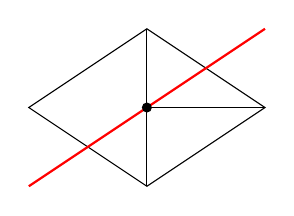
\begin{tikzpicture}[scale=1]

	% outline
	\draw (0,0) -- ++(1.5,-1) -- ++(1.5,1)-- ++(-1.5,1) -- cycle;
	\draw (1.5,-1) -- ++(0,2);
	\draw (1.5,0) -- ++(1.5,0);
	
	% red cross
	\draw[thick,red] (0,-1) --++ (3,2);

	% dot middle
	\filldraw (1.5,0) circle (1.6pt);

	\end{tikzpicture}

	\caption{not allowed}
	\label{ch1_triang_not_allowed}

\end{figure}	
	
	\item $V_h$ contains functions, which if restricted to $\tau$ are polynomials
	\item basis functions: $\varphi_i$ are simple to compute and have small support
\end{itemize}
\subsection{abstract finite element}
\begin{definition_}
	Finite elements in $R^d$ ($d\geq 1$) are triplets ($\tau,P_{\tau},\Sigma_{\tau}$) with 
	\begin{enumerate}[label=(\roman*)]
		\item $\tau \subset \R^d$ closed
		\item $P_{\tau}$ finite element space of functions: $\tau \to \R$, $n = \dim P_{\tau}$
		\item $\Sigma_{\tau}$ linearly independent, continuous functions $B_1,\dots,B_n:C^s(\tau) \to \R$, $s \in \N_0$ with $\forall \alpha_1, \dots, \alpha_n \in \R$ exists $p \in P_{\tau}$ s.t. $B_i (P) = \alpha_i$, $i = 1, \dots,n$
	\end{enumerate}
\end{definition_}
$B_i$ are the degrees of freedom (DoFs) of the finite element $p_i$ basis functions of the finite element. The space of all polynomials $\Omega \to R$ of degree $\leq k$ is $P_k$.

$d$-simplex $\tau \in \R^d$ is defined as convex hull of points $a_1,\dots,a_{d+1}\in R^{d+1}$.
\begin{equation*}
	\tau = \left\{ x\in \R^d: x= \displaystyle \sum^{d+1}_{i=1} \lambda_ia_i,\ 0 \leq \lambda_1, \dots,\lambda_{d+1}\leq 1,\ \displaystyle \sum^{d+1}_{i=1} \lambda_i =1\right\}
\end{equation*}
The $\lambda_i$ are called \glqq barycentric coordinates\grqq.
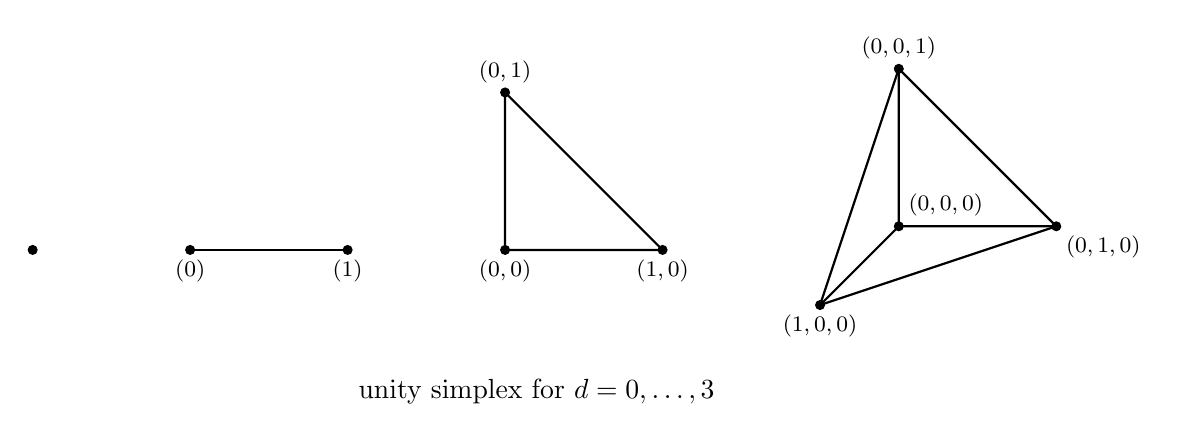
\begin{tikzpicture}[scale=2]
      \filldraw (0,0) circle (0.8pt);
%      \fill[black,font=\footnotesize] (0,0) node[below] {$(0)$};

      \draw[thick] (1,0) -- ++(1,0);
      \filldraw (1,0) circle (0.8pt);
      \filldraw (1,0) ++(1,0) circle (0.8pt);
      \fill[black,font=\footnotesize] (1,0) node[below] {$(0)$}
                                      (1,0) ++(1,0) node[below] {$(1)$};

      \draw[thick] (3,0) -- ++(0,1) -- ++(1,-1)--cycle;
      \filldraw (3,0)         circle (0.8pt);
      \filldraw (3,0) ++(1,0) circle (0.8pt);
      \filldraw (3,0) ++(0,1) circle (0.8pt);
      \fill[black,font=\footnotesize] (3,0)         node[below] {$(0,0)$}
                                      (3,0) ++(0,1) node[above] {$(0,1)$}
                                      (3,0) ++(1,0) node[below] {$(1,0)$};

      \draw[thick] (5.5,0.15) -- ++(0,1) --++(1,-1) -- cycle;
      \draw[thick] (5.5,0.15)  -- ++(-0.5,-0.5); -- ++(1.5,0.5);
      \draw[thick] (5.5,0.15) ++(0,1) -- ++(-0.5,-1.5) -- ++(1.5,0.5);
      \filldraw (5.5,0.15) circle (0.8pt);
      \filldraw (5.5,0.15) ++(0,1) circle (0.8pt);
      \filldraw (5.5,0.15) ++(1,0) circle (0.8pt);
      \filldraw (5.5,0.15) ++(-0.5,-0.5) circle (0.8pt);
      \fill[black,font=\footnotesize] (5.5,0.15) node[above right] {$(0,0,0)$}
                                      (5.5,0.15) ++(0,1) node[above] {$(0,0,1)$}
                                      (5.5,0.15) ++(1,0) node[below right] {$(0,1,0)$}
                                      (5.5,0.15) ++(-0.5,-0.5) node[below] {$(1,0,0)$};

%      \node at (3.2,-1.3) {Visualisierung des Einheitssimplex $T_n$ f\"ur $n=0,\dots,3$};
      \node at (3.2,-0.9) {unity simplex  for $d=0,\dots,3$};

    \end{tikzpicture}

\begin{example}
	\begin{enumerate}[label=(\roman*)]
		\item linear lagrange elements in $\R^d$
		\begin{equation*}
			P_{\tau} = P_1(\tau) = \left\{ p:\tau \to \R: p \text{ affin(=linear) in }\tau \right\} 
		\end{equation*}
		$\implies \dim P_{\tau} = d+1$.
		\begin{equation*}
			B_i(p) = p(a_i)\quad i = 1, \dots,d+1,\ p \in P_{\tau}
		\end{equation*}
		The basisfunctions are defined through
		\begin{equation*}
			p_j(a_i) = \delta_{ij} \quad i,j = 1,\dots ,d+1.
		\end{equation*}
		for \underline{$d=2$}, $\hat{\tau} \in \R^2$:
		\begin{equation*}
			a_1= (0,0),\ a_2 = (1,0),\ a_3 = (0,1)
		\end{equation*}
		see \eqref{tikz_unity_simplex}. This implies
		\begin{equation*}
			\begin{rcases}
			p_1(x,y) &= 1-x-y\\
			p_2(x,y) &= x\\
			p_3(x,y) &= y
			\end{rcases}
			(x,y) \in \hat{\tau}.
		\end{equation*} 
		\item quadratic lagrange elements in $\R^d$\\
		for \underline{$d=2$}, $\hat{\tau} \in \R^2$: $a_1,a_2,a_3$, vertices with midpoints $a_{ij} = \frac{1}{2}(a_i +a_j),\ i < j$.\\
		\begin{equation*}
			P_{\tau} = P_2(\tau) = \Big\{ p:\tau \to \R,\ p(x,y) = \alpha_1 + \alpha_2 x + \alpha_3 y + \alpha_4 xy + \alpha_5 x^2 + \alpha_6 y^2 \Big\}
		\end{equation*}
		$\implies  \dim P_{\tau} = 6$.
		\begin{equation*}
			\begin{rcases}
			B_i(p) &= p(a_i)\\
			B_{i+j+1}(p) &= p(a_{ij})
			\end{rcases}
			i,j = 1,2,3 \quad i<j
		\end{equation*}
		The basisfunctions are defined through 
		\begin{align*}
			p_j(a_i) &= \delta_{ij} &  i &=1,2,3, &  j&= 1,\dots,6\\
			p_j(a_{kl}) &= \delta_{k+l+1,j} &  k,l&=1,2,3\quad k<l &  j&=1,\dots,6 
		\end{align*}
		for $\hat{\tau} = \Big ( (0,0),(1,0),(0,1) \Big )$ we obtain e.g. for $p_2$:
		\begin{align*}
			p_2(0,0) &= 0 &  p_2(0,1) &= 0 &  p_2(0,\frac{1}{2})&= 0\\
			p_2(1,0) &= 1 &  p_2(\frac{1}{2},0) &= 0 &  p_2(\frac{1}{2},\frac{1}{2})&= 0.
		\end{align*}
		This gives a linear system to determine $\alpha_1,\dots,\alpha_6$.
		\begin{equation*}
			\implies p_2(x,y) = x(2x-1) \quad (x,y)\in \hat{\tau}.
		\end{equation*}
		\begin{figure}[H]
	\center
	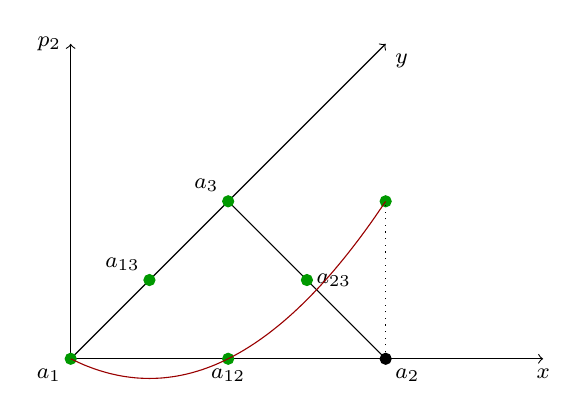
\begin{tikzpicture}[scale=2]

	\pgfmathsetmacro{\zerox}{0}
	\pgfmathsetmacro{\zeroy}{0}
	
	\pgfmathsetmacro{\ax}{\zerox + 2}
	\pgfmathsetmacro{\ay}{\zeroy + 1}
	
	
	% triangle
	\draw (\zerox,\zeroy) ++(2,0)-- ++(-1,1) --cycle;
	
	%axis
	\draw[->] (\zerox,\zeroy) -- ++(3,0);
	\draw[->] (\zerox,\zeroy) -- ++(0,2);
	\draw[->] (\zerox,\zeroy)  -- ++(2,2);
	\fill[black,font=\footnotesize] (\zerox,\zeroy) ++(3,0) node[below] {$x$}
									(\zerox,\zeroy) ++(2,2) node[below right] {$y$}
									(\zerox,\zeroy) ++(0,2) node[left] {$p_2$};
	
	% dots for a_2
	\filldraw (\zerox,\zeroy) ++(\ax,0) circle (1pt);
	\filldraw[green!60!black] (\ax,\ay) circle (1pt);
	\draw[dotted] (\zerox,\zeroy) ++(\ax,0)-- ++(0,\ay);
	
	% dots for a_i, a_{ij}
	\filldraw[green!60!black] (\zerox,\zeroy) circle (1pt);
	\filldraw[green!60!black] (\zerox,\zeroy) ++(1,1) circle (1pt);
	\filldraw[green!60!black] (\zerox,\zeroy) ++(1,0) circle (1pt);
	\filldraw[green!60!black] (\zerox,\zeroy) ++(0.5,0.5) circle (1pt);
	\filldraw[green!60!black] (\zerox,\zeroy) ++(1.5,0.5) circle (1pt);
	% nodes for for a_i, a_{ij}
	\fill[black,font=\footnotesize] (\zerox,\zeroy) node[below left] {$a_1$}
									(\zerox,\zeroy) ++(2,0) node[below right] {$a_2$}
									(\zerox,\zeroy) ++(1,1) node[above left] {$a_3$}
									(\zerox,\zeroy) ++(1,0) node[below] {$a_{12}$}
									(\zerox,\zeroy) ++(0.5,0.5) node[above left] {$a_{13}$}
									(\zerox,\zeroy) ++(1.5,0.5) node[right] {$a_{23}$};
	% linear parts
	%\draw[green!60!black] (\ax,\ay) -- ++(-1,-1.2); % line (a_2,1) to (a_12,0)
	%\draw[green!60!black] (\ax,\ay) -- ++(-0.5,-0.7); % line (a_2,1) to (a_23,0)
	%\draw[green!60!black] (\ax,\ay) -- ++(-0.75,-0.95); % line (a_2,1) to ???
	
	\draw[scale=2,domain=0:1,smooth,variable=\x,red!60!black] plot ({\x},{1/2*\x*(2*\x-1)});

	\end{tikzpicture}
		
	\caption{quadratic basisfunction $p_2$}
	\label{ch1_quadratic_basisfunction}

\end{figure}
		note that $p_2(x,\cdot)$ is constant. 
		\item cubic Hermite elements\\
		for \underline{$d=2$}, $\hat{\tau} \in \R^2$: $a_1,a_2,a_3, a_{123} = \frac{1}{3}(a_1+a_2+a_3)$
		\begin{figure}[H]
	\center
	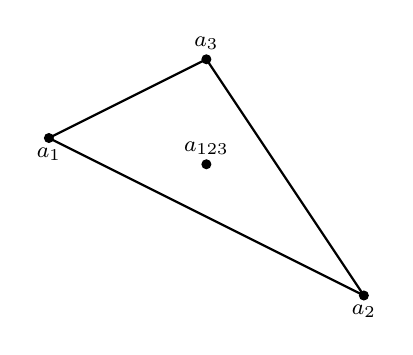
\begin{tikzpicture}[scale=2]


	\draw[thick] (0,0) -- ++(2,-1) -- ++(-1,1.5)--cycle;
	\filldraw (0,0)         circle (0.8pt);
	\filldraw (0,0) ++(2,-1) circle (0.8pt);
	\filldraw (0,0) ++(1,0.5) circle (0.8pt);
	\filldraw (0,0) ++(1,-1/6) circle (0.8pt);
	\fill[black,font=\footnotesize] (0,0) node[below] {$a_1$}
									(0,0) ++(2,-1) node[below] {$a_2$}
									(0,0) ++(1,0.5) node[above] {$a_3$}
									(0,0) ++(1,-1/6) node[above] {$a_{123}$};								
								
												

	\end{tikzpicture}
		
	\caption{Hermite element}
	\label{ch1_hermite_element}

\end{figure}
		\begin{align*}
		P_{\tau} = P_2(\tau) = \Big\{ p:\tau \to \R,\ p(x,y) &= \alpha_1 + \alpha_2 x + \alpha_3 y + \alpha_4 xy + \alpha_5 x^2 + \alpha_6 y^2 
		\\&\quad + \alpha_7x^2y +\alpha_8xy^2 +\alpha_9x^3 + \alpha_{10}y^3\Big\}
		\end{align*}
		$\implies \dim P_{\tau}= 10$
		\begin{equation*}
			\begin{rcases}
			B_i(p) &= p(a_i)\\
			B_4(p) &= p(a_{123})\\
			B_{i+4}(p) &= p_x(a_i)\\
			B_{i+7}(p) &= p_y(a_i)
			\end{rcases}
			i = 1,2,3
		\end{equation*}
		with $ p_x(a_i) =: \frac{\partial p}{\partial x}(a_i) $\\
		for $\hat{\tau} = \Big ( (0,0),(1,0),(0,1) \Big )$, $a_{123} = (\frac{1}{3},\frac{1}{3})$ we obtain e.g. for $p_5$ 
		\begin{align*}
			p_5(0,0) &= p_5(1,0) = p_5(0,1) = p_5(\frac{1}{3},\frac{1}{3}) = 0\\
			(p_5)_x(0,0) &= 1\\
			(p_5)_x(1,0) &= (p_5)_x(0,1) = 0\\
			(p_5)_y(0,0) &= (p_5)_y(0,0) = (p_5)_y(0,0) = 0
		\end{align*}
		$\implies$ $p_5(x,y) = x \left( 1 -3y -2x +3xy +x^2+2y^2 \right)$
	\end{enumerate}
\end{example}
\par
computation on $\hat{\tau}$ is relativly simple\\
\underline{idea}: transform each element $\tau$ to $\hat{\tau}$(reference element), also computation (integration) on $\hat{\tau}$ and transform back.\\
\begin{figure}[h!]
	\center
	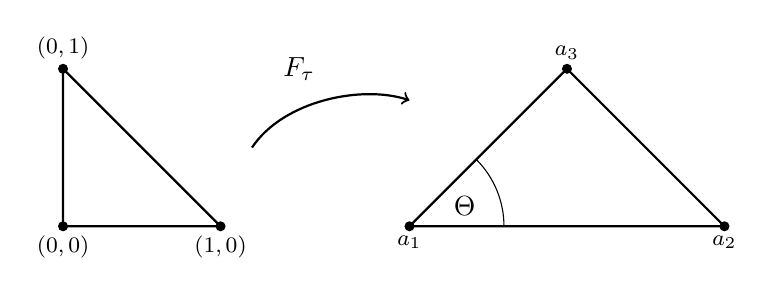
\begin{tikzpicture}[scale=2]

	
	


	% first simplix
	\draw[thick] (0,0) -- ++(0,1) -- ++(1,-1)--cycle;
	\filldraw (0,0)         circle (0.8pt);
	\filldraw (0,0) ++(1,0) circle (0.8pt);
	\filldraw (0,0) ++(0,1) circle (0.8pt);
	\fill[black,font=\footnotesize] (0,0) node[below] {$(0,0)$}
									(0,0) ++(1,0) node[below] {$(1,0)$}
									(0,0) ++(0,1) node[above] {$(0,1)$};
	
	%arrow
	\draw[thick,-to] (1.2,0.5) .. controls (1.4,0.8) and (1.9,0.9) .. (2.2, 0.8);
	
	%second simplex							
	\draw[thick] (2.2,0) -- ++(2,0) -- ++(-1,1)--cycle;
	\filldraw (2.2,0)         circle (0.8pt);
	\filldraw (2.2,0) ++(2,0) circle (0.8pt);
	\filldraw (2.2,0) ++(1,1) circle (0.8pt);
	\fill[black,font=\footnotesize] (2.2,0) node[below] {$a_1$}
									(2.2,0) ++(2,0) node[below] {$a_2$}
									(2.2,0) ++(1,1) node[above] {$a_3$};								
								
	
%	\pgfmathsetmacro{\ax}{2.2}
%	\pgfmathsetmacro{\ay}{0}
	
	\draw (2.2,0) ++(45:.6) arc (45:0:.6);
								
																		
	\node at (1.5,1) {$F_{\tau}$};
	\node at (2.55,0.13) {$\Theta$};				
	

	\end{tikzpicture}
		
	\caption{affine transformation}
	\label{ch1_plot_affin_equiv_triang}

\end{figure}
\begin{align*}
	&F_{\tau}: \hat{\tau} \to \tau\\
	&F_{\tau}(a) = Ba +b \quad B\in \R^{d\times d},\ b \in \R^d
\end{align*}
If $\hat{p}_i$ are basisfunctions on $\hat{\tau}$ we obtain 
\begin{equation*}
	p_i = \hat{p}_i \circ F^{-1}_{\tau},
\end{equation*}
$\tau = F_{\tau}(\hat{\tau})$ the basisfunctions on $\tau$.
\begin{align*}
	F_{\tau}(e_i) &= a_i, \qquad i=1,2,3\\
	F_{\tau}(a) &= (a_2-a_1,a_3-a_1)a + a_1\\
	B &=
	\begin{pmatrix}
	a_2-a_1\\
	a_3-a_1
	\end{pmatrix}
	,\quad a \in \hat{\tau}
\end{align*}
\begin{equation*}
	|\det B| = (a_2-a_1)(a_3-a_1)\sin \Theta
\end{equation*}
$\implies$
\begin{equation*}
	B(u,v) = 
	\begin{pmatrix}
	u_1 & v_1\\
	u_2 & v_2
	\end{pmatrix}
\end{equation*}
\begin{align*}
	(\det B)^2 & = (u_1v_2 - u_2v_1)^2\\
	& = (u^2_1+ u^2_2)(v^2_1+v^2_2)-(u_1v_1-u_2v_2)^2\\
	& = |u|^2|v|^2 - |u\cdot v|^2\\
	& = |u|^2|v|^2 (1- \cos \Theta)\\
	& = |u|^2|v|^2 \sin^2\Theta
\end{align*}
